

\subsection{Lattice setup}
    Gauge configurations in this work were obtained from the ensemble A40.24 which has been generated using $N_f = 2 + 1 + 1$ quark flavors. Details can be looked up in \cite{guage_configurations}.
    
    \begin{table}[h]
        \centering
        \begin{tabular}{lllllll}
        \hline
        \multicolumn{1}{|c|}{$\#$ used configurations} & \multicolumn{1}{c|}{$\beta$} & \multicolumn{1}{c|}{$\kappa$} & \multicolumn{1}{c|}{$a\mu_I$} & \multicolumn{1}{c|}{$a\mu_\sigma$} & \multicolumn{1}{c|}{$a\mu_\delta$} & \multicolumn{1}{c|}{$(L/a)^3 \times T$} \\ \hline
        \multicolumn{1}{|c|}{11} & \multicolumn{1}{c|}{3.9} & \multicolumn{1}{c|}{0.160856} & \multicolumn{1}{c|}{0.0040} & \multicolumn{1}{c|}{??} & \multicolumn{1}{c|}{??} & \multicolumn{1}{c|}{$24^3 \times 48$} \\ \hline
                               &                       &                       &                       &                       &                       &                       \\
                               &                       &                       &                       &                       &                       &                      
        \end{tabular}
        \caption{Parameters of gauge configurations used}
        \label{table_gauge_params}
    \end{table}
    % TODO explanation
    
\subsection{Meson masses}
    To investigate the accuracy and usefulness of the method of distillation described in this thesis comutations of charmonium state correlation functions where performed. These enable one to test different configurations of eigenvectors in relatively short times compared to the use of light doublet states. Beside the number of gauge configurations the number of eigenvectors can be arbitrarily set. In this section I will present the results for 2, 5 and 10 eigenvectors on the 11 gauge configurations mentioned in the previous section.\\
    
    In all computations the following creation operator was used:
    \begin{equation}
        \Operator(t) = \bar{\chi}^{(c)}(t)\gamma_5\chi^{(c)}(t)
    \end{equation}
    Therefore the resulting meson has quantum numbers $0(0^-)$. This was achieved by using for both propagators $(D^{-1(f)})$ the same flavor $f$. This approach reduced the amount of inversions that had to be calculated significantly. For the same reason a charmonium state was chosen in contrast to e.g. the calculation of a pion mass. Inversion for particles with higher masses converge significantly faster.
    
    \subsubsection{Result for 5 eigenvectors}
    In this section the result for a simulation with $N = 5$ will be presented all necessary steps discussed. In figure \ref{5_evs_full} the complete set of results from all 11 configurations can be seen.

    \begin{figure}[H]
        \centering
        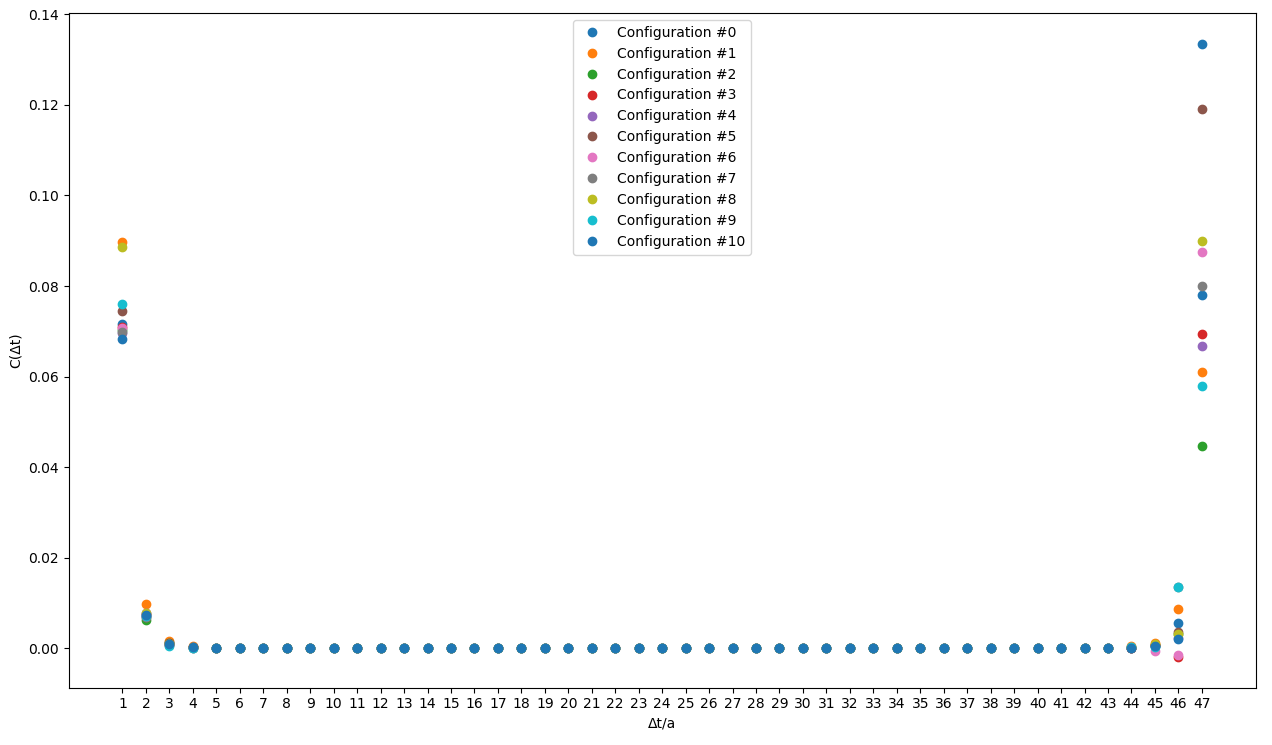
\includegraphics[width=1\textwidth]{images/5ev_all_configs.png} % first figure itself
        \caption{Data from all 11 configurations for 5 eigenvectors}
        \label{5_evs_full}
    \end{figure}
    
    To compute the mass of the charmonium state the mean value of all configurations for one value of $\Delta t$ were computed and a simple linear function was fitted to $ln(C(\Delta t))$. The results can be seen in figure \ref{5_evs_fit}. Using the same fitting parameters the exponential function on the left graph was calculated. Because the exponential nature of the correlation function only holds for $\Delta t \rightarrow \infty$ only a few points were chosen to be fitted. They can be recognized by a different color in both graphs.
    
     \begin{figure}[H]
        \centering
        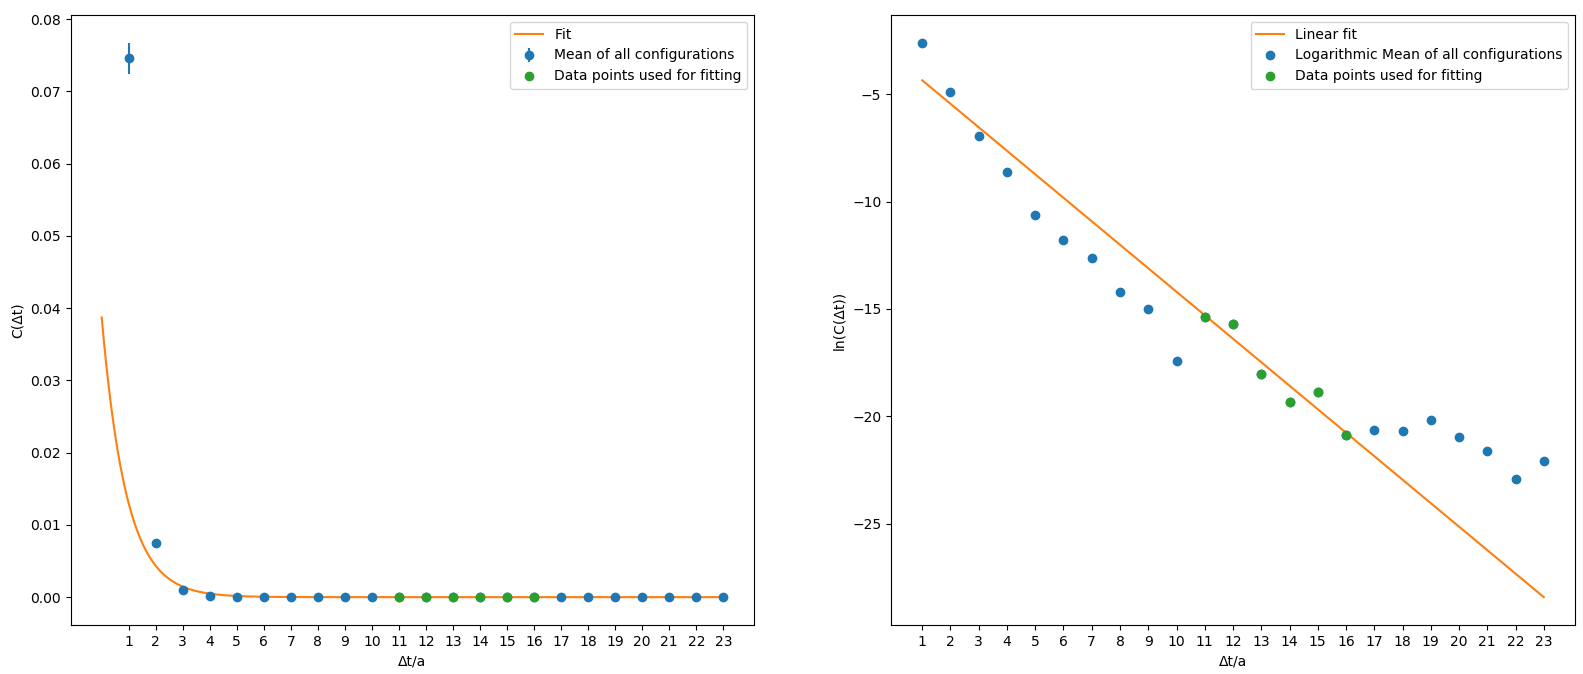
\includegraphics[width=1\textwidth]{images/5ev_fit.png} % first figure itself
        \caption{Fit to the mean values for 5 eigenvectors}
        \label{5_evs_fit}
    \end{figure}
    
    To calculate the fitting parameters and corresponding error the \textit{Jackknife}\cite{jackknife} method was used. The simulation with 5 eigenvectors produced the following result:
    $$ 2700 \text{MeV} \pm 45 \text{MeV} $$
    
    \subsubsection{Result for 2 and 10 eigenvectors}
    
    \begin{figure}[H]
        \centering
        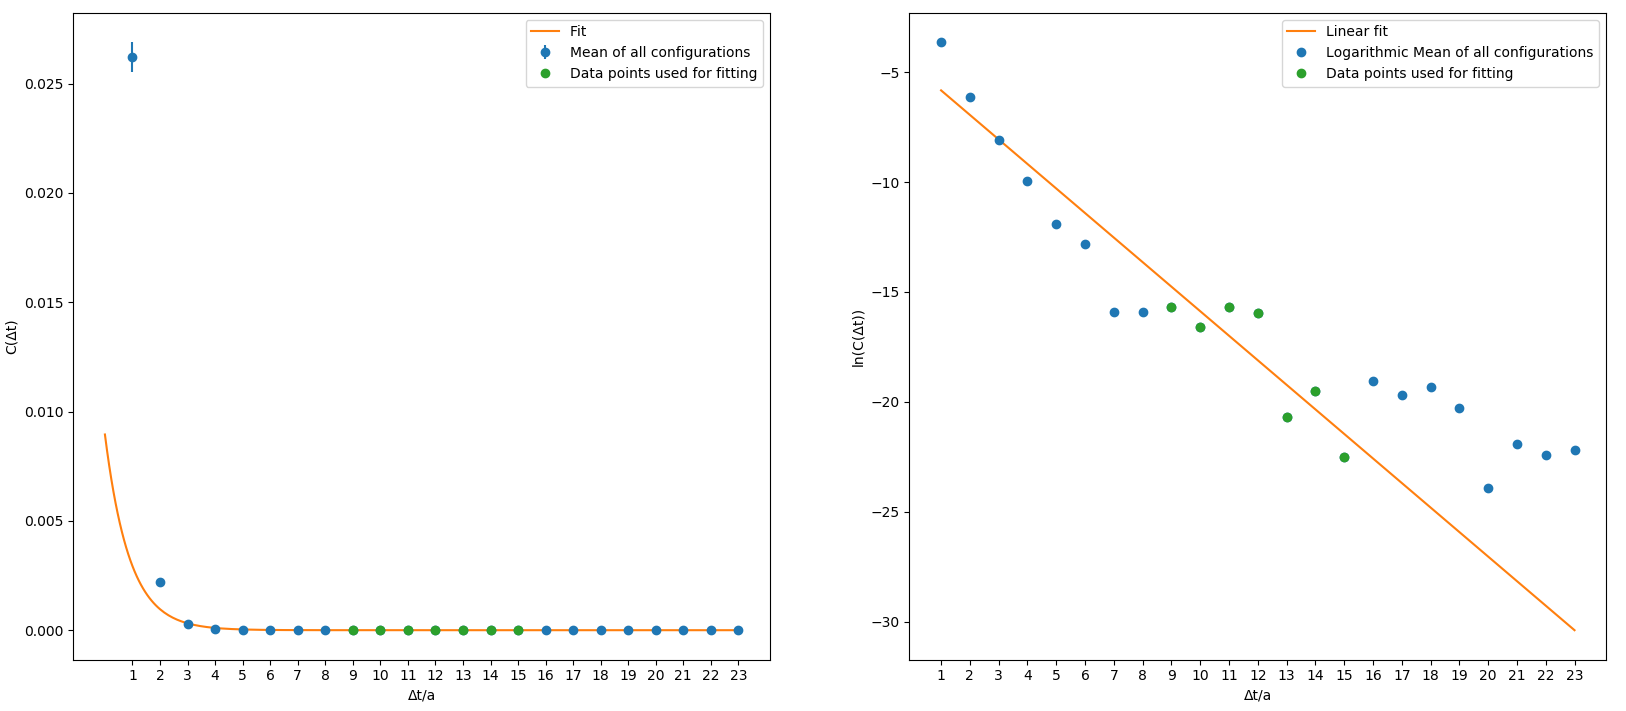
\includegraphics[width=1\textwidth]{images/2ev_fit.png} % first figure itself
        \caption{Fit to the mean values for 2 eigenvectors}
        \label{2_evs_fit}
    \end{figure}
    
    \begin{figure}[H]
        \centering
        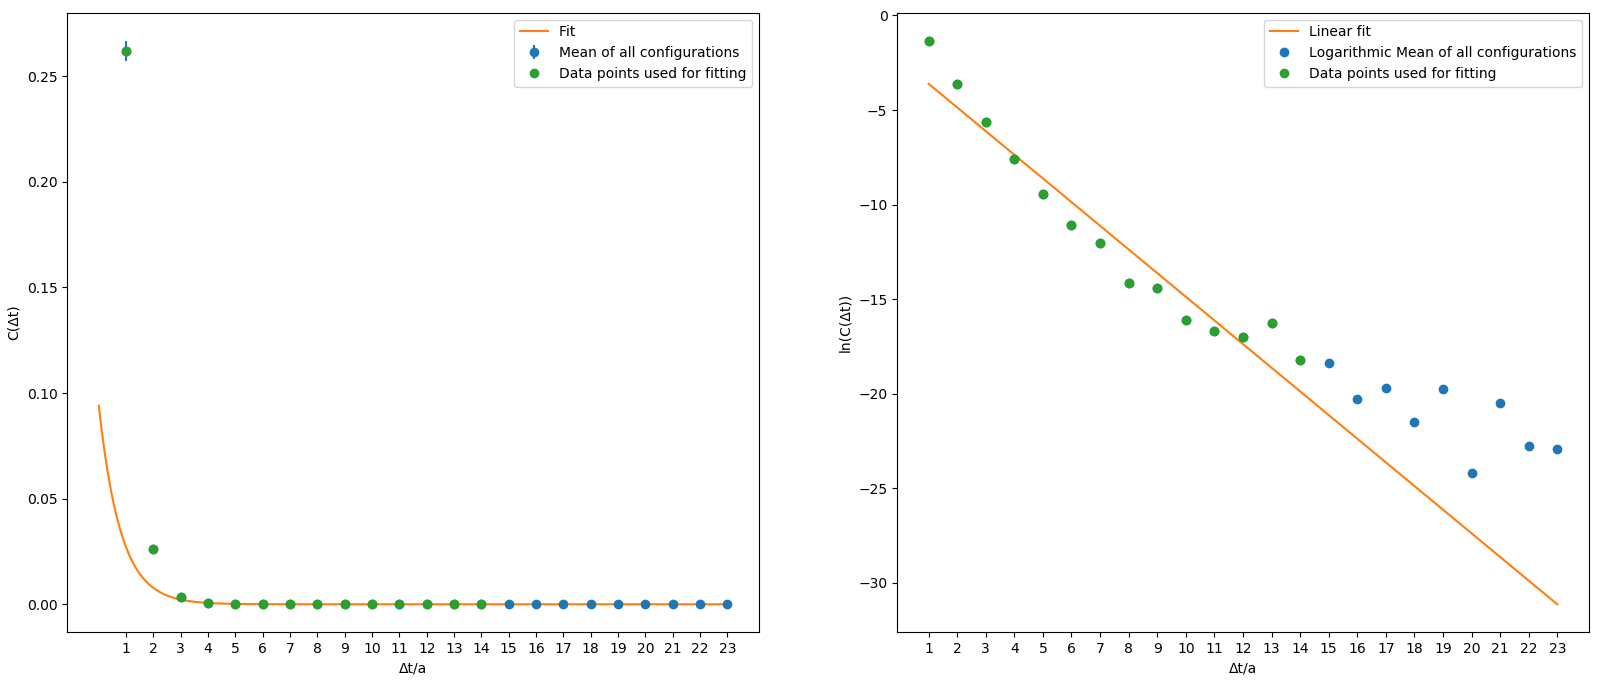
\includegraphics[width=1\textwidth]{images/10ev_fit.png} % first figure itself
        \caption{Fit to the mean values for 10 eigenvectors}
        \label{10_evs_fit}
    \end{figure}
    
    In figure \ref{2_evs_fit} and \ref{10_evs_fit} the results for 2 and 10 eigenvectors are presented respectively. When choosing the range of points to fit the function t ????. The result for 2 eigenvectors is:
    $$ 2752 \text{MeV} \pm 33 \text{MeV} $$
    For 10 eigenvector the simulation yielded:
    $$ 2501 \text{MeV} \pm 392 \text{MeV} $$